\section{Backend contribution}
The FastAPI backend provides the client authentication boundary, protected session resources, and the session-history surface consumed by the frontend. It enforces authenticated access before serving protected user resources.

\subsection{Authentication}
Authentication pages support sign-in, sign-up with email confirmation, and password reset through the AWS Amplify SDK and Cognito. Cognito and Google authentication were configured for the application.

The current security boundary is a one-time Cognito ID-token handoff to \texttt{/auth/session}. FastAPI validates the token and sets an HttpOnly application cookie. Subsequent protected API and SSE calls use same-origin cookie credentials; browser clients do not directly access DynamoDB or S3.

Figure~\ref{fig:cognito-auth-sequence} shows the direct Cognito registration path. The browser receives the Cognito ID token only for the one-time application-session bootstrap. The application session itself is the cookie set by FastAPI; the final protected requests therefore carry that cookie rather than a browser-managed bearer token.

\begin{figure}[H]
  \centering
  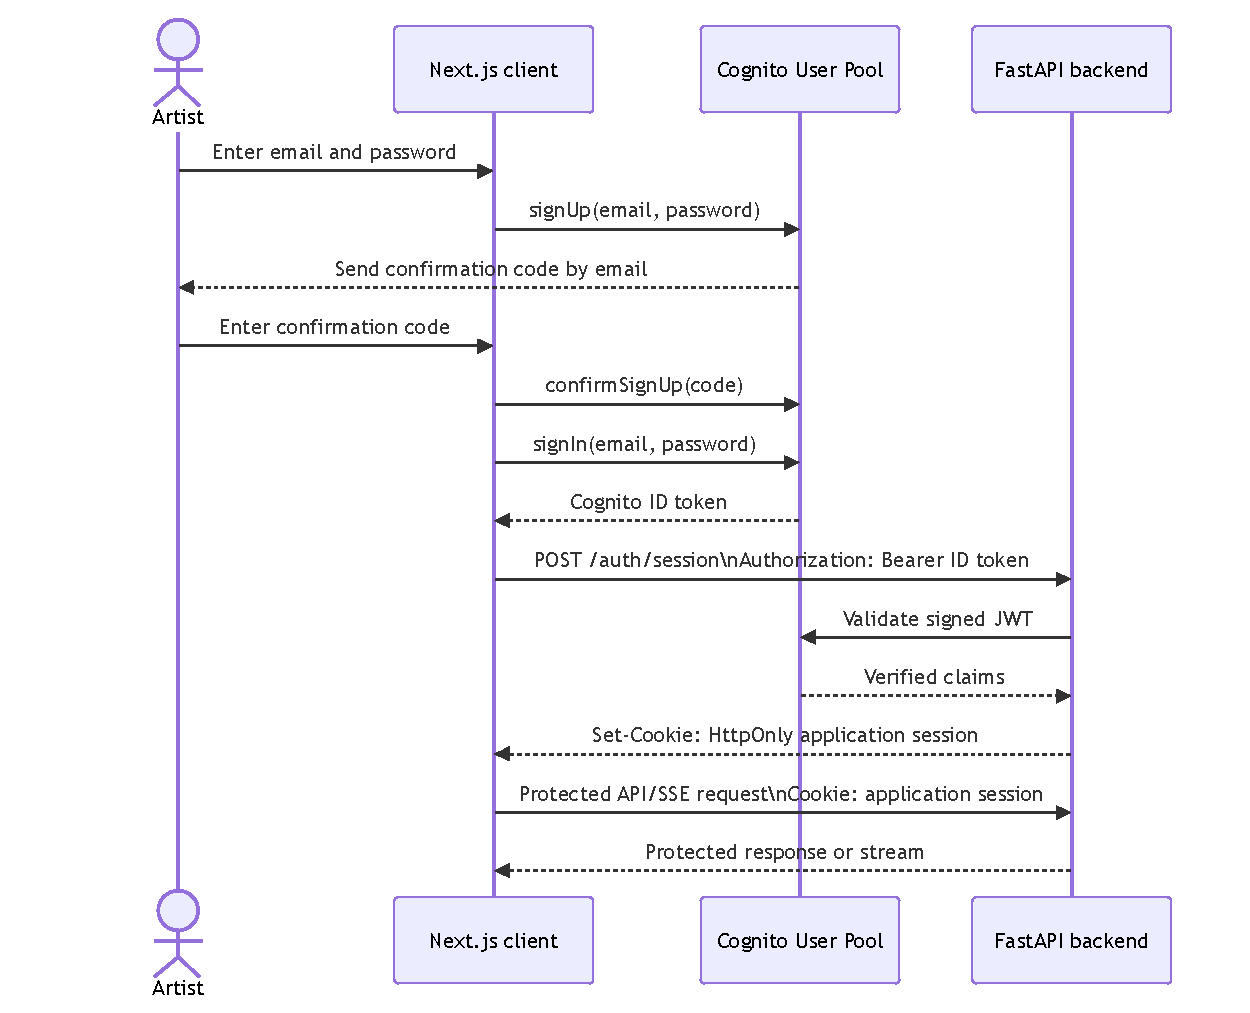
\includegraphics[width=\textwidth]{figures/authentication/cognito-auth-sequence.pdf}
  \caption{Direct Cognito sign-up, confirmation, and cookie-session bootstrap.}
  \label{fig:cognito-auth-sequence}
\end{figure}

Figure~\ref{fig:google-oauth-cookie} shows the corresponding Google OAuth route. Cognito's hosted UI mediates the provider redirect and code exchange. After Amplify obtains the Cognito ID token, the same FastAPI cookie-session bootstrap is used, so all subsequent protected client requests use the backend-issued cookie.

\begin{figure}[H]
  \centering
  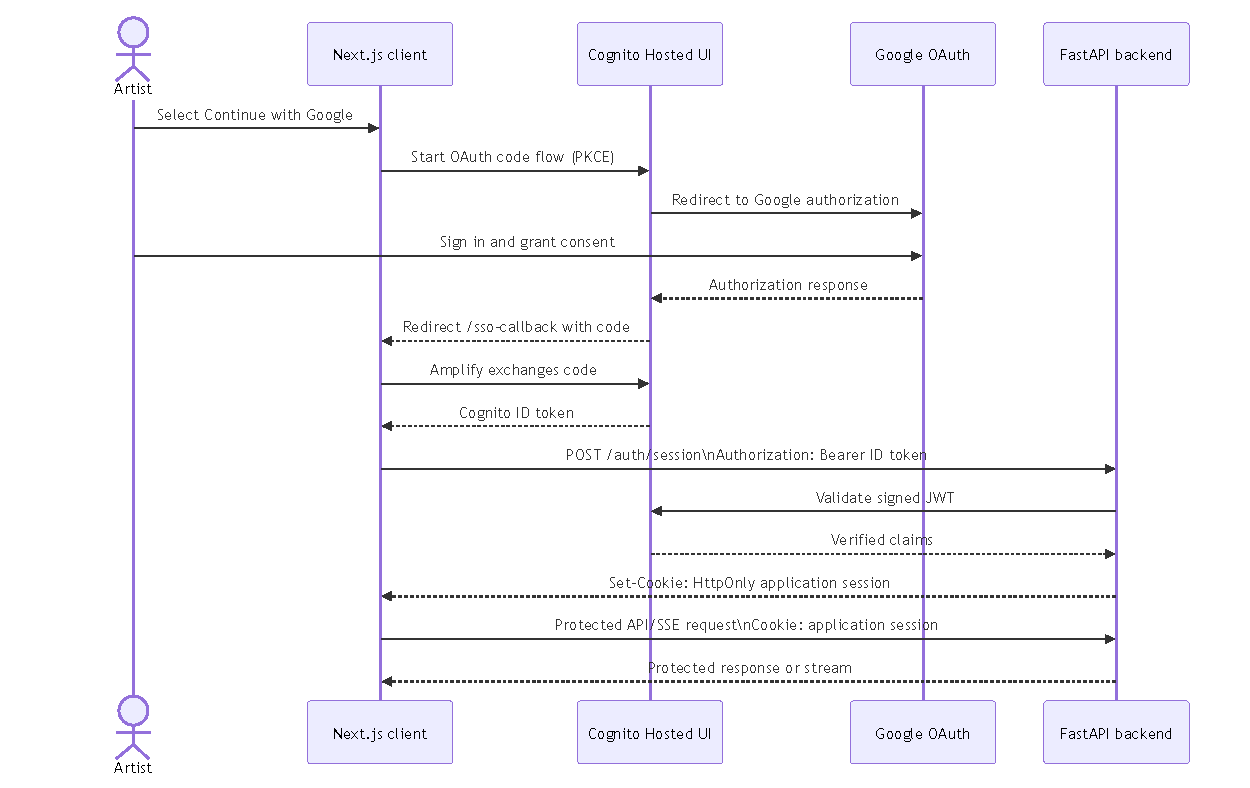
\includegraphics[width=\textwidth]{figures/authentication/google-oauth-cookie.pdf}
  \caption{Google OAuth through Cognito, followed by the same backend cookie-session boundary.}
  \label{fig:google-oauth-cookie}
\end{figure}
\clearpage

\subsection{Storage and session history}
Session metadata is owned by the authenticated user and supports sidebar history. Completed workspaces can be stored as a snapshot for later use. The detailed storage contributions and their recorded verification are listed in the Progress section.
